\documentclass[14pt]{beamer}
\usetheme{EastLansing}
\usecolortheme{spruce}

\usepackage{xcolor}
\usepackage{listings}
\usepackage{courier}
\usepackage{graphicx}
\usepackage{amsmath}
\usepackage{algorithm2e}
\usepackage{multicol}

% https://tex.stackexchange.com/questions/42619/x-mark-to-match-checkmark
\usepackage{pifont}% http://ctan.org/pkg/pifont

\usefonttheme[onlymath]{serif}

\definecolor{mGreen}{rgb}{0,0.6,0}
\definecolor{mGray}{rgb}{0.5,0.5,0.5}
\definecolor{mPurple}{rgb}{0.8,0,0.82}
\definecolor{backgroundColour}{rgb}{0.95,0.95,0.92}
\definecolor{lightBlue}{rgb}{0.1, 0.1, 0.8}

\newcommand\red[1]{{\color{red} #1}}
\newcommand\green[1]{{\color{green} #1}}

\newcommand{\cmark}{\ding{51}}%
\newcommand{\xmark}{\ding{55}}%

\lstdefinestyle{CStyle}{
    backgroundcolor=\color{backgroundColour},   
    commentstyle=\color{mGreen},
    keywordstyle=\color{magenta},
    numberstyle=\tiny\color{mGray},
    stringstyle=\color{mPurple},
    basicstyle=\footnotesize,
    breakatwhitespace=false,         
    breaklines=true,                 
    captionpos=b,                    
    keepspaces=true,                 
    numbers=left,                    
    numbersep=5pt,                  
    showspaces=false,                
    showstringspaces=false,
    showtabs=false,                  
    tabsize=2,
    language=C
}
\lstdefinestyle{pseudo}{
        basicstyle=\ttfamily\footnotesize,
        keywordstyle=\color{lightBlue},
        morekeywords={BEGIN,END,IF,ELSE,ENDIF,ELSEIF,PRINT,WHILE,RETURN,ENDWHILE,DO,FOR,TO,IN,ENDFOR,BREAK,INPUT},
        morecomment=[l]{//},
        commentstyle=\color{mGreen}
}

\lstset{basicstyle=\footnotesize\ttfamily,breaklines=true}
\lstset{framextopmargin=50pt,tabsize=2}

\title{ENGG1003 - Monday Week 2}
\subtitle{First steps: libraries \& modules, printing and plotting}
\author{Steve Weller}
\institute{University of Newcastle}
\date{\today}

\begin{document}
\titlepage

%==============================================================

\begin{frame}[fragile]
\frametitle{Lecture overview}
\begin{enumerate}
\item Python program with a library function \red{\S1.3}
	\begin{itemize}
		\item principles
		\item live demo
%		\item LL text \red{\S1.3}
	\end{itemize}
\item importing from modules and packages \red{\S1.4}
		\begin{itemize}
		\item principles
		\item live demo
	\end{itemize}
	
\item simple plotting \red{\S1.5} 
	\begin{itemize}
			\item principles
		\item live demo
%		\item %\& \red{\S1.8}
	\end{itemize}
	
\item plotting, printing and input data \red{\S1.6}
	\begin{itemize}
	\item principles
	\item live demo
%	\item 
	\end{itemize}
\end{enumerate}

\end{frame}

%==============================================================

\begin{frame}[fragile]
\frametitle{$1)$ Python program with a library function}
\begin{itemize}
\item describe the problem
\item simple diagram: $x, y, \theta$
\item maybe a ball?
\item algorithm is $\tan^{-1}$
\end{itemize}
\end{frame}

%==============================================================

\begin{frame}[fragile]
\frametitle{The program}

% screen grab of code from p.~12 text
\begin{figure}[ht]
	\centering
	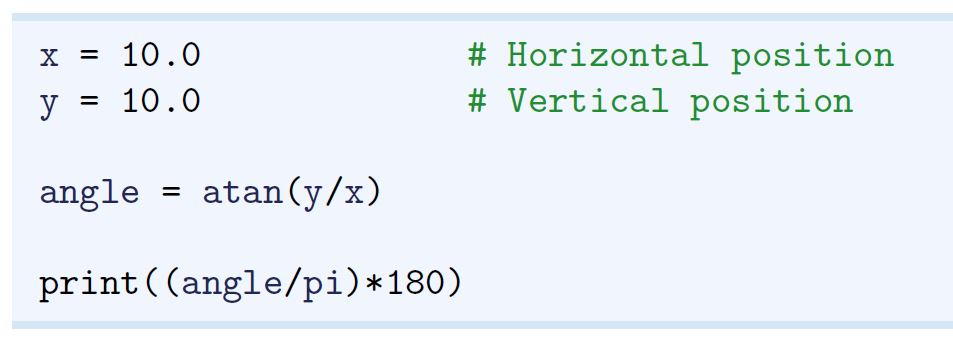
\includegraphics[width=\textwidth]{figures/LLp12}
\end{figure}

\begin{center}
\texttt{ball\_angle\_first\_try.py}
\end{center}

\end{frame}

%==============================================================

\begin{frame}[fragile]
\frametitle{First use of a Python function}
\begin{itemize}
\item first use of a \red{\emph{function}}, in this case \texttt{atan}
\item \red{\emph{argument}}
\item \red{\emph{return value}}
\end{itemize}

\end{frame}

%==============================================================

\begin{frame}[fragile]
\frametitle{Math review: radians and degrees}
\begin{itemize}
\item Python's \texttt{atan} returns value in radians
\item $\times \frac{180}{\pi}$ to get answer in degrees
\end{itemize}
\end{frame}

%==============================================================

\begin{frame}[fragile]
\frametitle{Running the program}
\begin{itemize}
\item screen grab from PyCharm -- error message
\end{itemize}
\end{frame}

%==============================================================

\begin{frame}[fragile]
\frametitle{Python standard library and import}
\begin{itemize}
\item Python has plenty of functionality ``built-in''
\item LOTS more can be \red{\emph{imported}}
\item \texttt{atan} and other trigonometric functions not built in
\item to activate that functionality, must explicitly import
\item \texttt{atan} function is grouped together with many other mathematical functions in a \red{\emph{library module}}  called \texttt{math}
\end{itemize}

% screen grab of code from p.~13 text
\begin{figure}[ht]
	\centering
	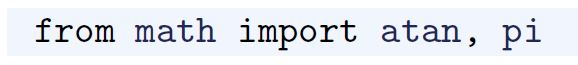
\includegraphics[width=0.6\textwidth]{figures/LLp13a}
\end{figure}

\end{frame}

%==============================================================

\begin{frame}[fragile]
\frametitle{The program: second attempt}

% screen grab of code from p.~13 text
\begin{figure}[ht]
	\centering
	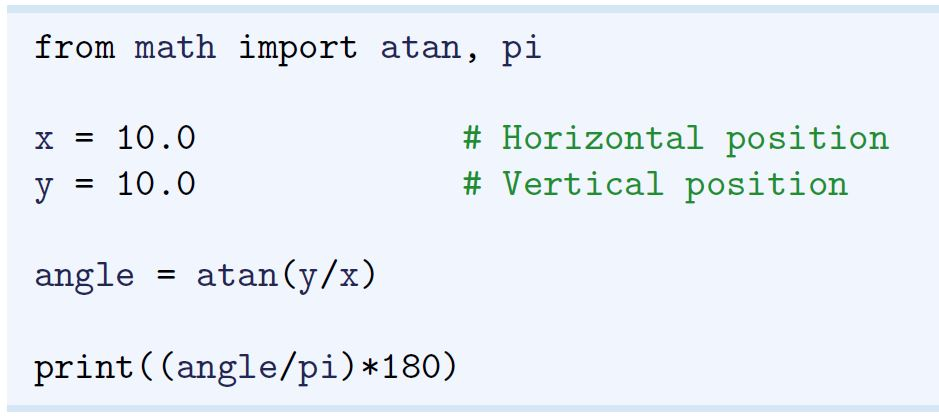
\includegraphics[width=0.9\textwidth]{figures/LLp13b}
\end{figure}
\begin{center}
\texttt{ball\_angle.py}
\end{center}
\begin{itemize}
\item script correctly produces $45.0$ as output
\item live demo in PyCharm shortly
\end{itemize}

\end{frame}

%==============================================================

\begin{frame}[fragile]
\frametitle{Another way of importing}
\begin{itemize}
\item use the import statement import math, but require \texttt{atan} and \texttt{pi} to be \red{\emph{prefixed}} with math
\item both techniques are commonly used and are the two basic ways of importing library code in Python
%\item Importing code is an evident part of Python programming, so we better shed some more light on it
\end{itemize}
\begin{figure}[ht]
	\centering
	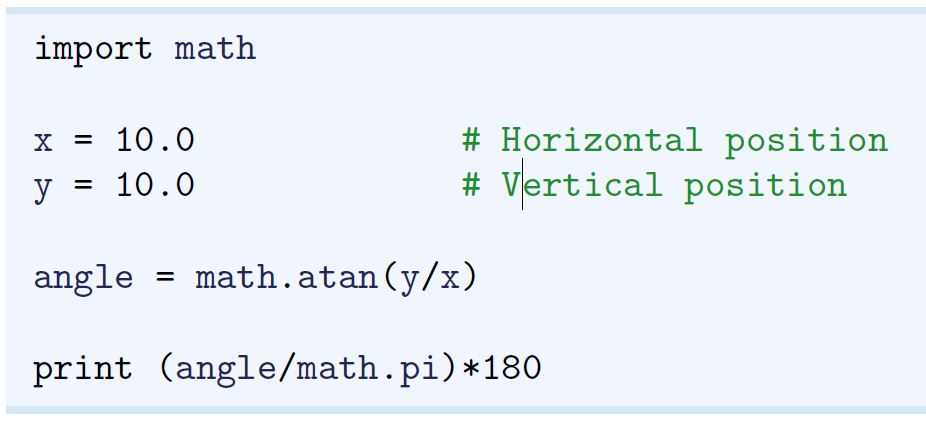
\includegraphics[width=0.7\textwidth]{figures/LLp14}
\end{figure}
\vspace*{-5mm}
\begin{center}
\texttt{ball\_angle\_prefix.py}
\end{center}

\end{frame}

%==============================================================

\begin{frame}[fragile]
\frametitle{Live demo of Python program with a library function}
blah
\end{frame}

%==============================================================

\begin{frame}[fragile]
\frametitle{$2)$ Importing from modules and packages}

motivation and context

%At first, it may seem cumbersome to have code in different libraries, since it means
%you have to know (or find out) what resides in which library.10 Also, there are
%many libraries around in addition to the Python standard library itself. To your
%comfort, you come a long way with just a few libraries, and for easy reference, the
%handful of libraries used in this book is listed below (Sect. 1.4.5). Having everything
%available at any time would be convenient, but this would also mean that computer
%memory would be filled with a lot of unused information, causing less memory to be
%available for computations on big data. Python has so many libraries, with so much
%functionality, that importing what is needed is indeed a very sensible strategy.

\begin{itemize}
\item[(a)] importing for use \textbf{\emph{without}} prefix %, eg: \texttt{ball\_angle.py}

\item[(b)] importing for use \textbf{\emph{with}} prefix %, eg: \texttt{ball\_angle\_prefix.py}
\end{itemize}

\end{frame}

%==============================================================

\begin{frame}[fragile]
\frametitle{Importing for use \emph{without} prefix}

% screen grab of code from p.~13 text
\begin{figure}[ht]
	\centering
	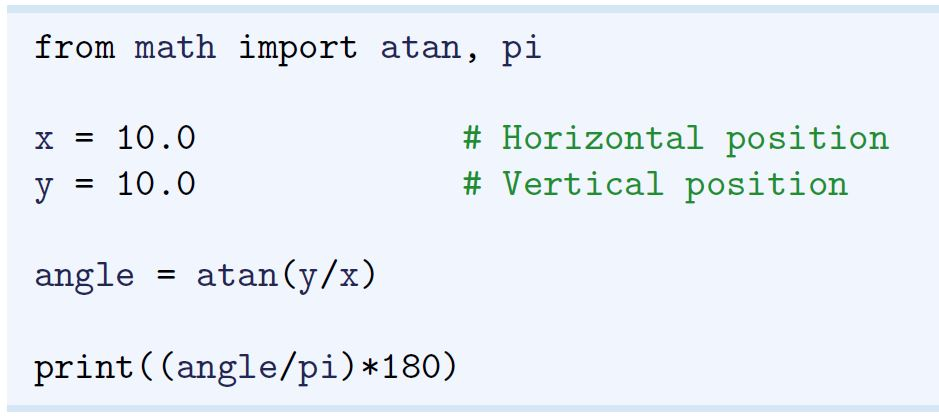
\includegraphics[width=0.8\textwidth]{figures/LLp13b}
\end{figure}
\begin{itemize}
\item[\green{\cmark}] Python code is easier to read
\item[\red{\xmark}] allows name conflicts!
\end{itemize}

%\cmark

\end{frame}

%==============================================================

\begin{frame}[fragile]
\frametitle{Name conflicts}
\begin{itemize}
\item explain the basic idea
\item do \emph{not} explain example from text, which is too complicated
\item will show an example shortly
\end{itemize}

\end{frame}

%==============================================================

\begin{frame}[fragile]
\frametitle{Importing for use \emph{with} prefix}

% screen grab of code from p14 text
\begin{figure}[ht]
	\centering
	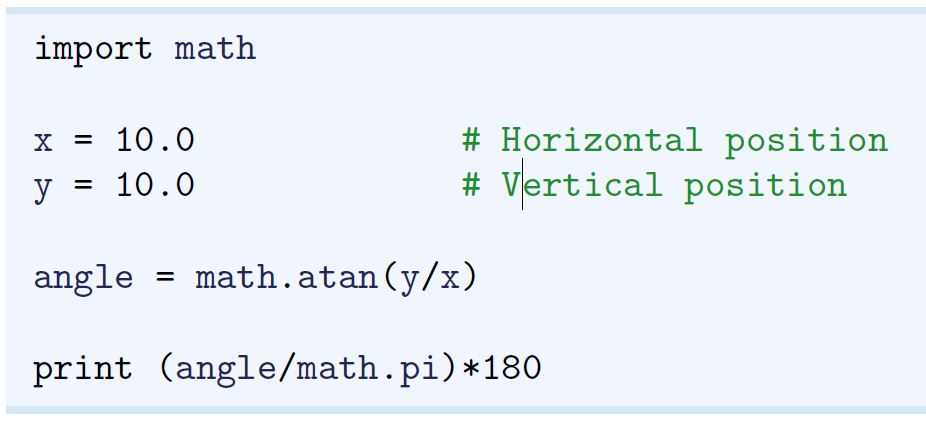
\includegraphics[width=0.8\textwidth]{figures/LLp14}
\end{figure}
\begin{itemize}
\item[\red{\xmark}] Python code is a little harder for humans to read
\item[\green{\cmark}\green{\cmark}] eliminates name conflicts!
\item \textbf{standard and safer and preferred method of importing}
\end{itemize}

\end{frame}

%==============================================================

\begin{frame}[fragile]
\frametitle{Avoiding name conflict using prefixes}

% screen grab of code from p17 text
\begin{figure}[ht]
	\centering
	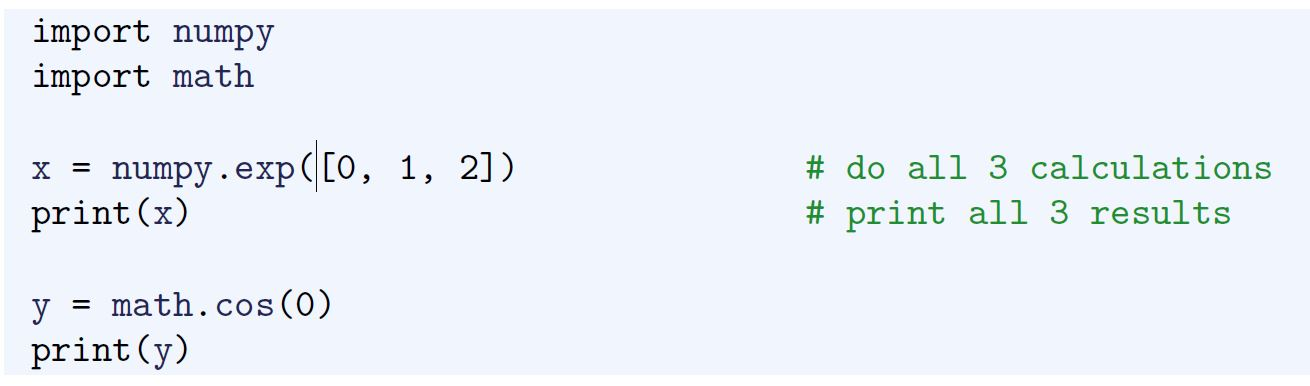
\includegraphics[width=0.8\textwidth]{figures/LLp17}
\end{figure}
\begin{itemize}
	\item \texttt{numpy} library includes an \texttt{exp} function
	\begin{itemize}
		\item math review:~exponential function $e^{z} =$~\texttt{exp(z)}
	\end{itemize}
	\item \texttt{math} library also includes an \texttt{exp} function---with a different implementation!
	\item[\green{\cmark}] \textbf{prefixes make clear which \texttt{exp} to use}
\end{itemize}

\end{frame}

%==============================================================

\begin{frame}[fragile]
\frametitle{Imports with name change}

% screen grab of code from p18 text
\begin{figure}[ht]
	\centering
	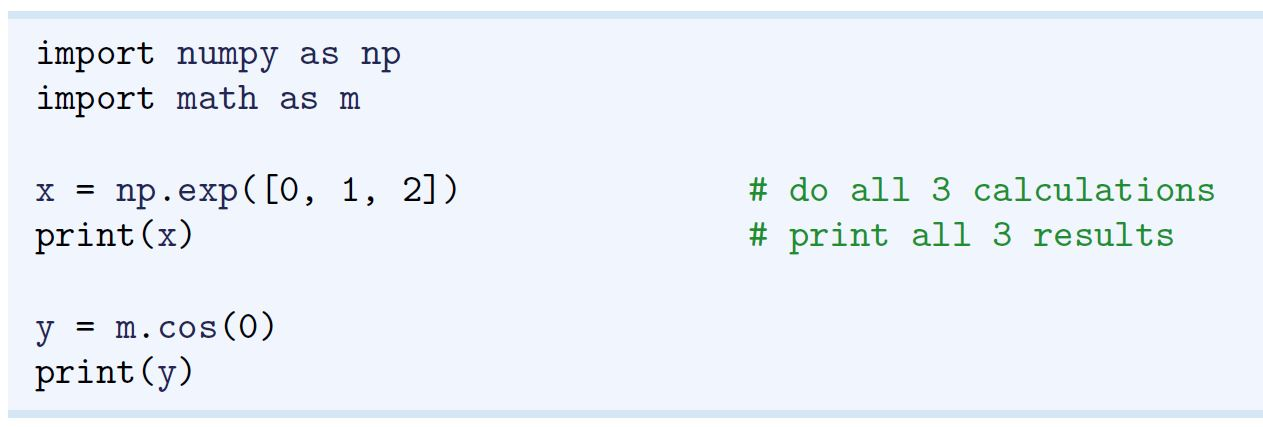
\includegraphics[width=0.9\textwidth]{figures/LLp18}
\end{figure}
\vspace*{-8mm}
\begin{itemize}
\item using \red{as}, \texttt{numpy} name becomes \texttt{np} 
\item similar for \texttt{math} and \texttt{m}
\item[\green{\cmark}] Python code is easy to read
\item[\green{\cmark}\green{\cmark}] eliminates name conflicts
\end{itemize}

\end{frame}

%%==============================================================
%
%\begin{frame}[fragile]
%\frametitle{Importing from packages}
%\begin{itemize}
%\item xxx
%\end{itemize}
%
%\end{frame}
%
%%==============================================================
%
%\begin{frame}[fragile]
%\frametitle{}
%\begin{itemize}
%\item xxx
%\end{itemize}
%
%\end{frame}

%%==============================================================
%
%\begin{frame}[fragile]
%\frametitle{}
%\begin{itemize}
%\item xxx
%\end{itemize}
%
%\end{frame}

%==============================================================

\begin{frame}[fragile]
%\frametitle{Main modules \& packages used in ENGG1003}
\frametitle{Main modules used in ENGG1003}
\begin{itemize}
\item \texttt{math}---description
\item \texttt{numpy}---description
\item \texttt{matplotlib}---description
%\item \texttt{random}---description
%\item \texttt{sympy}---description
%\item \texttt{timeit}---description
%\item \texttt{sys}---description
\end{itemize}

%math—see, e.g., ball_angle.py, Sect. 1.3.
%• numpy—see, e.g., check_functions.py above.
%• matplotlib.pyplot—see, e.g., ball_plot.py, Sect. 1.5.
%• random—see, e.g., throw_2_dice.py in Sect. 2.4.
%• sympy—see, e.g., Sect. 5.3.
%• timeit—see, e.g., Sect. 5.6.
%• sys—see, e.g., Sect. 7.2.2.


\end{frame}

%%==============================================================
%
%\begin{frame}[fragile]
%\frametitle{}
%\begin{itemize}
%\item xxx
%\end{itemize}
%
%\end{frame}

%==============================================================

\begin{frame}[fragile]
\frametitle{Live demo of importing from modules and packages}
blah
\end{frame}

%==============================================================

\begin{frame}[fragile]
\frametitle{3) Simple plotting}
blah
\end{frame}

%==============================================================

\begin{frame}[fragile]
\frametitle{Live demo of simple plotting}
blah
\end{frame}

%==============================================================

\begin{frame}[fragile]
\frametitle{4) Plotting, printing and input data}
blah
\end{frame}

%==============================================================

\begin{frame}[fragile]
\frametitle{Live demo of plotting, printing and input data}
blah
\end{frame}

\end{document}
